
\documentclass{standalone}

% additional header file for standalone images


\usepackage{tikz}
\usepackage{tikz-3dplot}
\usetikzlibrary{patterns, shapes}
\usepackage{pgfplots}
\pgfplotsset{compat=1.16}
\usetikzlibrary{cd}

\newcommand{\LTRIA}{0.5}
\newcommand{\triang}[2]{\filldraw[fill=#2!60!white, draw=#2!50!black, very thick] #1 -- ($ #1 + (\LTRIA, 0) $) -- ($ #1 + (0.5*\LTRIA, \LTRIA) $) -- cycle;}

\newcommand{\BZRc}{0.5519}

\newcommand{\bezierc}[2] {
  \begin{scope}[cm={#1,0,0,#1,(0,0)}]
  \draw[very thick, #2] (0,1) .. controls (\BZRc, 1) and (1,\BZRc) .. (1,0);
  \draw[very thick, #2] (1,0) .. controls (1, -\BZRc) and (\BZRc, -1) .. (0,-1);
  \draw[very thick, #2] (0,-1) .. controls (-\BZRc, -1) and (-1,-\BZRc) .. (-1,0);
  \draw[very thick, #2] (-1,0) .. controls (-1, \BZRc) and (-\BZRc,1) .. (0,1);
\end{scope}
}

\newcommand{\beziercnl}[3] {
  \begin{scope}[cm={#1,0,0,#1,(0,0)}]
    \draw[very thick, #3] (0,1.2) .. controls (\BZRc, 1.2) and ($(1,\BZRc)-(#2,0.0)$) .. (1,0);
    \draw[very thick, #3] (1,0) .. controls ($(1, -\BZRc)+(#2,0.0)$) and ($(\BZRc, -1) + (0.0,#2)$) .. (0,-1.1);
    \draw[very thick, #3] (0,-1.1) .. controls ($(-\BZRc, -1)-(0.0,#2)$) and ($(-1.2,-\BZRc)-(#2,0.0)$) .. (-1,0);
    \draw[very thick, #3] (-1,0) .. controls ($(-.8, \BZRc)+(#2,0.0)$) and (-\BZRc,1.2) .. (0,1.2);
\end{scope}
}

\newcommand{\beziercnlTwo}[4] {
  \begin{scope}[cm={#1,0,0,#1,(0,0)}]
    \coordinate (Pnorth) at ($(0, 1.2) + (0, #4)$);

    \draw[very thick, #3] (Pnorth) .. controls ($(\BZRc, 0) + (Pnorth)$) and ($(1,\BZRc)-(#2,0.0)$) .. (1,0);
    \draw[very thick, #3] (1,0) .. controls ($(1, -\BZRc)+(#2,0.0)$) and ($(\BZRc, -1) + (0.0,#2)$) .. (0,-1.1);
    \draw[very thick, #3] (0,-1.1) .. controls ($(-\BZRc, -1)-(0.0,#2)$) and ($(-1.2,-\BZRc)-(#2,0.0)$) .. (-1,0);
    \draw[very thick, #3] (-1,0) .. controls ($(-.8, \BZRc)+(#2,0.0)$) and ($(-\BZRc,0)+(Pnorth)$) .. (Pnorth);
\end{scope}
}


\begin{document}
	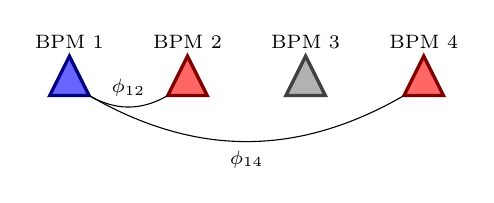
\begin{tikzpicture}
	%	\draw[thick] (-1,-1) -- (5.5,-1) -- (5.5,1.5) -- (-1,1.5) -- cycle;

    \triang{(0,0)}{blue}
    \triang{(1.5,0)}{red}
    \triang{(3,0)}{gray}
    \triang{(4.5,0)}{red}
    \scriptsize
    \node[above] at ($ (\LTRIA*0.5,\LTRIA) $) {BPM 1};
    \draw (\LTRIA,0) to[bend right] (1.5,0);
    \node at (1,0.1) {$ \phi_{12} $};
    
    \node[above] at ($ (1.5+\LTRIA*0.5,\LTRIA) $) {BPM 2};
    \draw ($(\LTRIA,0)$) to[bend right] (4.5,0);
    \node[below] at ($(2.25+\LTRIA*0.5,-.6)$) {$ \phi_{14} $};
    
    \node[above] at ($ (3+\LTRIA*0.5,\LTRIA) $) {BPM 3};
    
    \node[above] at ($ (4.5+\LTRIA*0.5,\LTRIA) $) {BPM 4};
	\normalsize
	\end{tikzpicture}
\end{document}